%!TeX encoding = UTF-8
%!TeX program = xelatex
\documentclass[notheorems, aspectratio=54]{beamer}
% aspectratio: 1610, 149, 54, 43(default), 32
\usepackage[utf8]{inputenc} % `utf8` option to match Editor encoding
\usepackage[T1]{fontenc}
\usepackage{latexsym}
\usepackage{amsmath,amssymb}
\usepackage{mathtools}
\usepackage{color,xcolor}
\usepackage{graphicx}
\usepackage{algorithm}
\usepackage{amsthm}
\usepackage{lmodern} % 解决 font warning
% \usepackage[UTF8]{ctex}
\usepackage{animate} % insert gif
\usepackage{listings}

\usepackage{karnaugh-map}

\usetikzlibrary{matrix,calc}
\usepackage{lipsum} % To generate test text 
\usepackage{ulem} % 下划线,波浪线

\usepackage{listings} % display code on slides; don't forget [fragile] option after \begin{frame}


% ----------------------------------------------
% tikx
\usepackage{framed}
\usepackage{tikz}
\usepackage{pgf}
\usetikzlibrary{calc,trees,positioning,arrows,chains,shapes.geometric,%
    decorations.pathreplacing,decorations.pathmorphing,shapes,%
    matrix,shapes.symbols}
\pgfmathsetseed{1} % To have predictable results
% Define a background layer, in which the parchment shape is drawn
\pgfdeclarelayer{background}
\pgfsetlayers{background,main}

% define styles for the normal border and the torn border
\tikzset{
  normal border/.style={black!70!gray, decorate, 
     decoration={random steps, segment length=2.5cm, amplitude=.7mm}},
  torn border/.style={black!70!gray, decorate, 
     decoration={random steps, segment length=.5cm, amplitude=1.7mm}}}

% Macro to draw the shape behind the text, when it fits completly in the
% page
\def\parchmentframe#1{
\tikz{
  \node[inner sep=2em] (A) {#1};  % Draw the text of the node
  \begin{pgfonlayer}{background}  % Draw the shape behind
  \fill[normal border] 
        (A.south east) -- (A.south west) -- 
        (A.north west) -- (A.north east) -- cycle;
  \end{pgfonlayer}}}

% Macro to draw the shape, when the text will continue in next page
\def\parchmentframetop#1{
\tikz{
  \node[inner sep=2em] (A) {#1};    % Draw the text of the node
  \begin{pgfonlayer}{background}    
  \fill[normal border]              % Draw the ``complete shape'' behind
        (A.south east) -- (A.south west) -- 
        (A.north west) -- (A.north east) -- cycle;
  \fill[torn border]                % Add the torn lower border
        ($(A.south east)-(0,.2)$) -- ($(A.south west)-(0,.2)$) -- 
        ($(A.south west)+(0,.2)$) -- ($(A.south east)+(0,.2)$) -- cycle;
  \end{pgfonlayer}}}

% Macro to draw the shape, when the text continues from previous page
\def\parchmentframebottom#1{
\tikz{
  \node[inner sep=2em] (A) {#1};   % Draw the text of the node
  \begin{pgfonlayer}{background}   
  \fill[normal border]             % Draw the ``complete shape'' behind
        (A.south east) -- (A.south west) -- 
        (A.north west) -- (A.north east) -- cycle;
  \fill[torn border]               % Add the torn upper border
        ($(A.north east)-(0,.2)$) -- ($(A.north west)-(0,.2)$) -- 
        ($(A.north west)+(0,.2)$) -- ($(A.north east)+(0,.2)$) -- cycle;
  \end{pgfonlayer}}}

% Macro to draw the shape, when both the text continues from previous page
% and it will continue in next page
\def\parchmentframemiddle#1{
\tikz{
  \node[inner sep=2em] (A) {#1};   % Draw the text of the node
  \begin{pgfonlayer}{background}   
  \fill[normal border]             % Draw the ``complete shape'' behind
        (A.south east) -- (A.south west) -- 
        (A.north west) -- (A.north east) -- cycle;
  \fill[torn border]               % Add the torn lower border
        ($(A.south east)-(0,.2)$) -- ($(A.south west)-(0,.2)$) -- 
        ($(A.south west)+(0,.2)$) -- ($(A.south east)+(0,.2)$) -- cycle;
  \fill[torn border]               % Add the torn upper border
        ($(A.north east)-(0,.2)$) -- ($(A.north west)-(0,.2)$) -- 
        ($(A.north west)+(0,.2)$) -- ($(A.north east)+(0,.2)$) -- cycle;
  \end{pgfonlayer}}}

% Define the environment which puts the frame
% In this case, the environment also accepts an argument with an optional
% title (which defaults to ``Example'', which is typeset in a box overlaid
% on the top border
\newenvironment{parchment}[1][Example]{%
  \def\FrameCommand{\parchmentframe}%
  \def\FirstFrameCommand{\parchmentframetop}%
  \def\LastFrameCommand{\parchmentframebottom}%
  \def\MidFrameCommand{\parchmentframemiddle}%
  \vskip\baselineskip
  \MakeFramed {\FrameRestore}
  \noindent\tikz\node[inner sep=1ex, draw=black!20, fill=black!90, 
          anchor=west, overlay] at (0em, 2em) {\sffamily#1};\par}%
{\endMakeFramed}

% ----------------------------------------------

\mode<presentation>{
    \usetheme{Warsaw}
    % Boadilla CambridgeUS
    % default Antibes Berlin Copenhagen
    % Madrid Montpelier Ilmenau Malmoe
    % Berkeley Singapore Warsaw
    \usecolortheme{seagull}
    % beetle, beaver, orchid, whale, dolphin, seagull
    \useoutertheme{infolines}
    % infolines miniframes shadow sidebar smoothbars smoothtree split tree
    \useinnertheme{circles}
    % circles, rectanges, rounded, inmargin
}

% ---------------------------------------------------------------------
% Jet Black Theme
\setbeamercolor{normal text}{fg=white,bg=black!90}
\setbeamercolor{structure}{fg=white}

\setbeamercolor{alerted text}{fg=red!85!black}

\setbeamercolor{item projected}{use=item,fg=black,bg=item.fg!35}

\setbeamercolor*{palette primary}{use=structure,fg=structure.fg}
\setbeamercolor*{palette secondary}{use=structure,fg=structure.fg!95!black}
\setbeamercolor*{palette tertiary}{use=structure,fg=structure.fg!90!black}
\setbeamercolor*{palette quaternary}{use=structure,fg=structure.fg!95!black,bg=black!80}

\setbeamercolor*{framesubtitle}{fg=white}

\setbeamercolor*{block title}{parent=structure,bg=black!70!gray}
\setbeamercolor*{block body}{fg=black,bg=black!10}
\setbeamercolor*{block title alerted}{parent=alerted text,bg=black!15}
\setbeamercolor*{block title example}{parent=example text,bg=black!15}
% ---------------------------------------------------------------------


% ---------------------------------------------------------------------
% flow chart
\tikzset{
    >=stealth',
    punktchain/.style={
        rectangle, 
        rounded corners, 
        % fill=black!10,
        draw=white, very thick,
        text width=6em,
        minimum height=2em, 
        text centered, 
        on chain
    },
    largepunktchain/.style={
        rectangle,
        rounded corners,
        draw=white, very thick,
        text width=10em,
        minimum height=2em,
        on chain
    },
    line/.style={draw, thick, <-},
    element/.style={
        tape,
        top color=white,
        bottom color=blue!50!black!60!,
        minimum width=6em,
        draw=blue!40!black!90, very thick,
        text width=6em, 
        minimum height=2em, 
        text centered, 
        on chain
    },
    every join/.style={->, thick,shorten >=1pt},
    decoration={brace},
    tuborg/.style={decorate},
    tubnode/.style={midway, right=2pt},
    font={\fontsize{10pt}{12}\selectfont},
}
% ---------------------------------------------------------------------

% code setting
\lstset{
    language=C++,
    basicstyle=\ttfamily\footnotesize,
    keywordstyle=\color{red},
    breaklines=true,
    xleftmargin=2em,
    numbers=left,
    numberstyle=\color[RGB]{222,155,81},
    frame=leftline,
    tabsize=4,
    breakatwhitespace=false,
    showspaces=false,               
    showstringspaces=false,
    showtabs=false,
    morekeywords={Str, Num, List},
}

% ---------------------------------------------------------------------

\newcommand{\reditem}[1]{\setbeamercolor{item}{fg=red}\item #1}

% 缩放公式大小
\newcommand*{\Scale}[2][4]{\scalebox{#1}{\ensuremath{#2}}}

% 解决 font warning
\renewcommand\textbullet{\ensuremath{\bullet}}

% -------------------------------------------------------------

%% preamble
\title[Wskaźniki]{Wskaźniki}
% \subtitle{The subtitle}
\author{Adam Djellouli}

% -------------------------------------------------------------

\begin{document}

% title frame
\begin{frame}
    \titlepage
\end{frame}

\begin{frame}
Wskaźniki:
\begin{itemize}
\item są najważniejszym narzędziem w C/C++ (wiele popularnych języków nie dopuszcza bezpośredniego działania na wskaźnikach);
\item umożliwiają konstrukcje struktur danych;
\item pozwalają na tworzenie szybkiego i wydajnego kodu;
\item są niezbędne do dynamicznej alokacji pamięci.
\end{itemize}

\end{frame}

\begin{frame}[fragile]
O co w tym chodzi?
\center
\begin{table}[!htb]
\begin{minipage}{.5\linewidth}
\begin{figure}

  \includegraphics[width=0.9\linewidth]{pudlo}
\end{figure}
\end{minipage}%
\begin{minipage}{.5\linewidth}

\begin{lstlisting}
int A = 139;
int *wsk = &A;
\end{lstlisting}
~\\
Zmienna - pudełko z imieniem, do którego możemy włożyć jakąś wartość (liczbę, napis, wartość logiczną).\\~\\
Wskaźnik - zmienna, która trzyma informacje o tym gdzie w pamięci siedzi inna zmienna.

\end{minipage} 
\end{table}

\end{frame}


\begin{frame}[fragile]
Dlaczego wskaźnik musi mieć typ?\\
Nie wszystkie pudełka mają taki sam rozmiar.\\
Wskaźnik umożliwa nam skoczenie do pudełka za i przed, musi więc wiedzieć jak daleko ma skoczyć.
\begin{center}
\begin{tabular}{ |c |c | }
 \hline
 typ & ilość miejsca \\ 
\hline
 char & 1 \\ 
 short & 2 \\  
 int, long, float & 4 \\
 double & 8  \\
\hline
\end{tabular}
~\\~\\
\flushleft
Jak to sprawdzić?
\begin{lstlisting}
printf("%d", sizeof(short));
\end{lstlisting}

\end{center}

\end{frame}

\begin{frame}[fragile]
Wskaźniki, a tablice
\center
\begin{table}[!htb]
\begin{minipage}{.5\linewidth}
\begin{figure}

  \includegraphics[width=0.9\linewidth]{tablice}
\end{figure}
\end{minipage}%
\begin{minipage}{.5\linewidth}

\begin{lstlisting}
int *p;
int a[3] = {2,0,5};
p = &a[0];
int* p2 = p + 1;
\end{lstlisting}
~\\
Zmienne w tablicy przechowywane są obok siebie.\\
Możemy przypisać wskaźnikowi adres dowolnej zmiennej w tablicy, a następnie przesunąć się do innych elementów używając dodawania lub odejmowania.\\
Co się stanie jeśli w ten sposób wyjdziemy poza granice naszej tablicy?\\
\end{minipage} 
\end{table}
\end{frame}

\begin{frame}[fragile]
Odejmowanie wskaźników\\

Różnica wskaźników to liczba półek jakie się znajdują między półkami, na które wskazują.

\begin{lstlisting}
int a[] = {6, 2, 10};
int *p0 = a;
int *p1 = a+1;
int *p2 = a+2;
printf("p2-p0: %d\n",p2-p0); // p2-p0: 2
printf("p2-p1: %d\n",p2-p1); // p2-p1: 1
printf("p0-p1: %d\n",p0-p1); // p0-p1: -1
\end{lstlisting}

\end{frame}

\begin{frame}[fragile]
Cyz wskaźnik może nie wskazywać na nic?\\
Może i często chcemy żeby tak było.
\begin{lstlisting}
int *p;
p = NULL;
\end{lstlisting}

Przypisanie wartości NULL spowoduje, że wskaźnik nie będziena nic wskazywał.\\
Dwa pusta wskaźniki są zawsze równe, stąd przydatność do wyznaczania granic różnych struktur.
\begin{figure}

  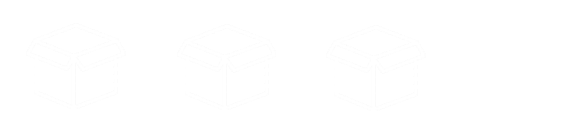
\includegraphics[width=0.9\linewidth]{lista}
\end{figure}

\end{frame}

\begin{frame}[fragile]
Operatory wskaźników\\
Czyli znaczki, które cos zrobią gdy użyjemy je razem ze wskaźnikiem.\\
\center
\begin{tabular}{ |c |c | c |}
\hline
 znaczek & co to robi? & przykład \\ 
\hline
 $*$ & deklaracja wskaźnika & $int *p;$ \\ 
\hline
 $*$ & wyłuskanie wartości na którą wskazuje & $printf(" \% d", *p);$ \\ 
\hline

$+-$ & inkrementacja \textbackslash dekremntacja & $p = p + 1;$ \\ 
\hline
 $==, !=$ & porównanie dwóch wskaźników & $if(p == NULL)$ \\ 
\hline

\end{tabular}


\end{frame}


\begin{frame}
Czego nie należy robić ze wskaźnikami?\\
\begin{itemize}
\item Wskaźniki nigdy nie powinny być używane przed inicjalizacją.\\
\item Odwoływanie się do wskaźnika do którego nie przydzielono pamięci.\\
\item Mylenie znaczków i zamienne stosowanie wskaźników i zmiennych na które wskazują.\\
\item Wyjechanie wskaźnikiem za tablicę.
\end{itemize}


\end{frame}


\end{document}